\section{Question 2: Dataset 2}

%Something here

\subsection{Data Preproccessing}

First of all, we import data from the day.csv file.
The dataset contains 731 observations with 16 columns, including factors such as weather conditions, seasonal information, temperature, and rental counts.

Dataset Overview Date Range: The data spans from January 1, 2011, to December 31, 2012.
Key Variables: season : season (1:springer, 2:summer, 3:fall, 4:winter) workingday : if day is neither weekend nor holiday is 1, otherwise is 0.
temp: Normalized temperature in Celsius.
atemp: Normalized feeling temperature in Celsius.
hum: Normalized humidity.
windspeed: Normalized wind speed.
casual: Count of casual users.
registered: Count of registered users.
cnt: Total count of bike rentals (sum of casual and registered).

In this report, we choose to analyze the relationship between total number of rentals due to environment settings.
Therefore we will skip the following collumn: instant, date


\begin{table}[ht]
\centering
\begin{tabular}{lllllrrrrrr}
  \hline
  season & holiday & weekday & workingday & weathersit & temp & atemp & hum & windspeed & registered & cnt \\ 
  \hline
 1 & 0 & 4 & 1 & 2 & 0.40 & 0.40 & 0.67 & 0.19 & 3571 & 3761 \\ 
   4 & 0 & 5 & 1 & 1 & 0.36 & 0.36 & 0.54 & 0.21 & 5283 & 5992 \\ 
   2 & 0 & 1 & 1 & 1 & 0.53 & 0.53 & 0.59 & 0.18 & 3698 & 4362 \\ 
   2 & 0 & 3 & 1 & 2 & 0.62 & 0.58 & 0.77 & 0.10 & 4494 & 5260 \\ 
   2 & 0 & 0 & 0 & 1 & 0.61 & 0.57 & 0.51 & 0.23 & 4286 & 7132 \\ 
   4 & 0 & 3 & 1 & 2 & 0.48 & 0.47 & 0.72 & 0.15 & 3490 & 3894 \\ 
   \hline
\end{tabular}
\end{table}

\subsubsection{Missing data}

According to the author description, there is no missing value in this dataset, so it is not a problem that we should care for.

\subsubsection{Dependent variables choosing}

Because of a few factors, we chose to use registered as our dependent variable: registered is one of the 3 dependent variables that we can choose and all other variables yr, season, holiday, workingday, weathersit, mnth have some relation with registered in an acceptable level.

\subsubsection{Outlier}

\begin{figure}[H]
\centering
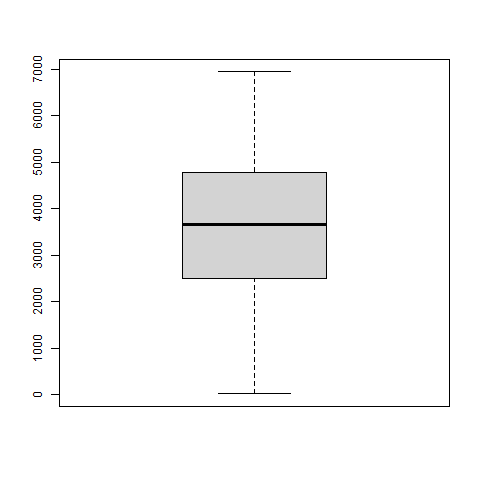
\includegraphics[scale=.4]{img/registered_box_plot.png}
\caption{Box plot of registered}
\label{fig:registered_box_plot}
\end{figure}

Looking at the box plot, we can see that there is no outliers for our dependent variable.

\subsection{Data overview}
First of all, we might want to look at the summary table contain the statistic descriptive to have the overview about our dataset.

\begin{table}[ht]
\centering
\begin{tabular}{lllllll}
  \hline
         &      temp &     atemp &      hum &   windspeed &   registered &      cnt \\ 
  \hline
      Min& 0.05913& 0.07907& 0.0000& 0.02239& 20& 22\\ 
        1st Qu.& 0.33708& 0.33784& 0.5200& 0.13495& 2497& 3152\\ 
          Median& 0.49833& 0.48673& 0.6267& 0.18097& 3662& 4548\\ 
          Mean& 0.49538& 0.47435& 0.6279& 0.19049& 3656& 4504\\ 
           3rd Qu.& 0.65542& 0.60860& 0.7302& 0.23321& 4776& 5956\\ 
           Max& 0.86167& 0.84090& 0.9725& 0.50746& 6946& 8714\\ 
            &  &  &  &  &  &  \\ 
   \hline
\end{tabular}
\end{table}


\subsubsection{Key Observations:}

\begin{itemize}
    \item \textbf{Variation}: The continuous variables show significant variation, particularly \textbf{humidity} and \textbf{windspeed}.
    \item \textbf{Central Tendency}: The mean and median values for most variables are close, indicating a relatively symmetrical distribution.
    \item \textbf{Range}: The wide range in values for \textbf{registered} indicates days with both low and high rental counts.
\end{itemize}
This summary provides a good foundation for further analysis, such as examining relationships between variables or identifying potential outliers.

 


\subsection{Data deepdive}
To have a deeper look about our dataset and how the variable actually related with each other, we will have to look at the correlation heatmap plot, which was conducted to identify relationships between numeric variables

\begin{figure}[H]
\centering
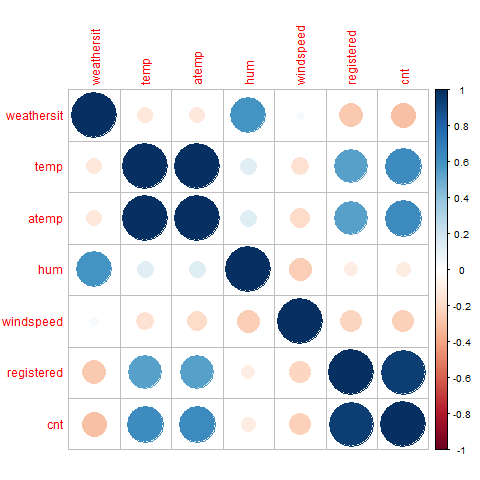
\includegraphics[width=0.7\textwidth]{img/corplot.png}
\caption{Correlation Matrix}
\label{fig:Correlation_matrix_Q2_2}
\end{figure}

We can observe that there is a strong correlation in some variables, especially between temp and atemp.

\subsection{Data splitting}

The data is split into two part, training dataset and validation dataset. Training dataset contains 80$\%$ of the observations and the validation dataset contains 80$\%$ of the observations. The split is performed randomly with RStudio.

For replication, we use the seed 777489.

\subsection{Building baseline model}

From the above section we can see that temp and atemp have a strong relationship. Below is a plot that describe how much the relation is:

\begin{figure}[H]
\centering
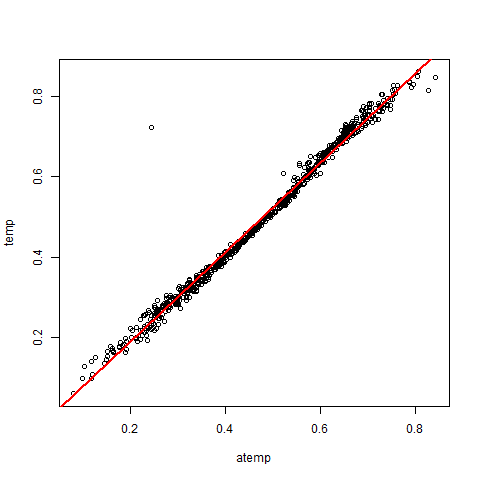
\includegraphics[width=0.7\textwidth]{img/temp_atemp.png}
\caption{Relation between temp and atemp}
\label{fig:relation_between_temp_and_atemp}
\end{figure}


As we can see from the plot, temp and atemp have a strong linear relationship. Therefore, we will not use atemp in our model.

In our decription, holiday and workingday and weekday also have strong relation. If it is a holiday then it is not a working day and weekday is 6 it also not a workingday.  

To choose which one we will include in our baseline model, we look on how much they impact to the registered through box-plot.

\begin{figure}[H]
\centering
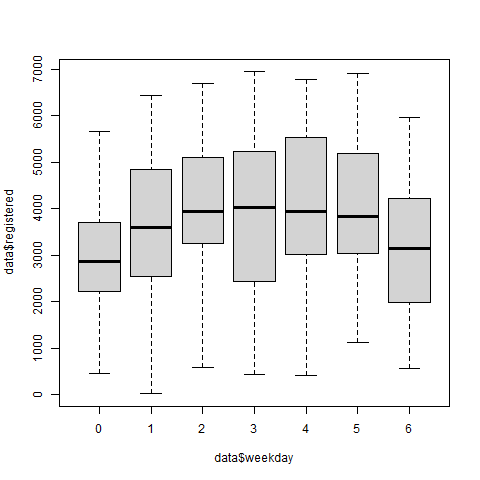
\includegraphics[width=0.55\textwidth]{img/weekday.png}
\caption{Impact of Weekday}
\label{fig:scaled_revenue_distribution}
\end{figure}

\begin{figure}[H]
\centering
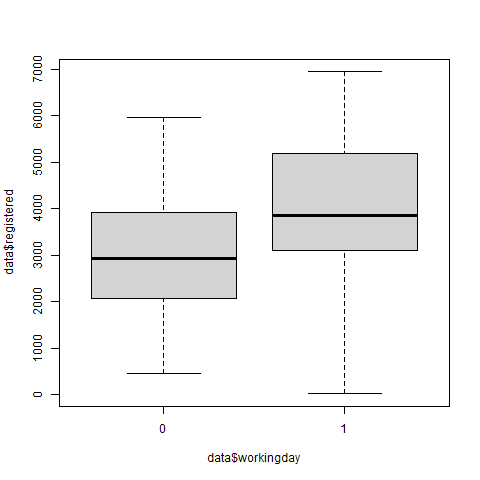
\includegraphics[width=0.55\textwidth]{img/workingday.png}
\caption{Impact of Workingday}
\label{fig:scaled_revenue_distribution}
\end{figure}

\begin{figure}[H]
\centering
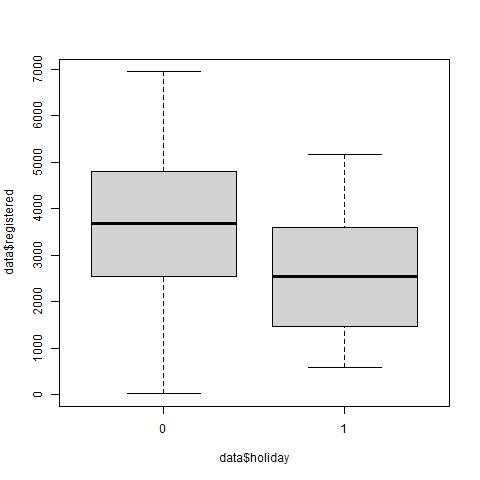
\includegraphics[width=0.55\textwidth]{img/holiday.png}
\caption{Impact of holiday}
\label{fig:scaled_revenue_distribution}
\end{figure}

From the definition, we can clearly figure out that when weekday is 0 or 6, working day is 0, this lead to multicollinearity. Consider that the impact of the weekday is not more significant than the other two, we decide not to use this variable in out model.

temp:
\begin{figure}[H]
\centering
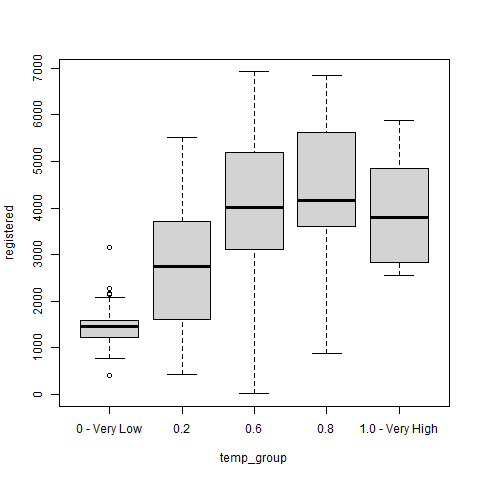
\includegraphics[width=0.55\textwidth]{img/plottemp3.png}
\caption{Impact of temp}
\label{fig:scaled_revenue_distribution}
\end{figure}

People tend to use rental bicycles more when temperature is warmer but not too hot. 

Humidity:
\begin{figure}[H]
\centering
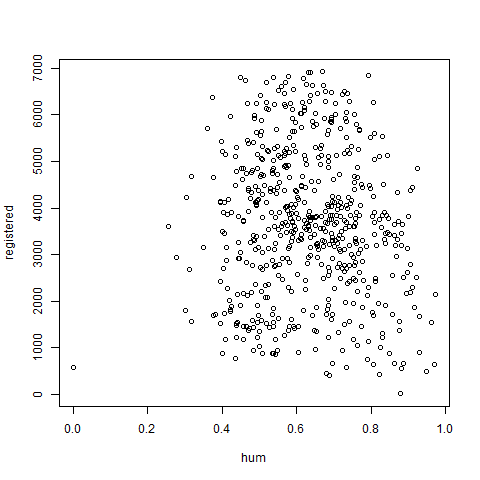
\includegraphics[width=0.55\textwidth]{img/plothum.png}
\caption{Plot of how registered depend on humidity}
\label{fig:humidity_on_registered_plot}
\end{figure}

As we can see, most of the data collected is in range [0.4,0.8] and humidity is clearly have relation on registered, so we are going to keep it.

Similarly, we will keep windspeed, season and yr, mnth (we may want to eliminate them later)
We have our first baseline model

\begin{center}
    $registered = \beta_1 \ + \ \beta_2 \ holiday \ + \ \beta_3 \ yr \ + \ \beta_{4,i} \ mnth_i \ + \ \beta_{5,j} \ weathersit_j \ + \ \beta_6 \ temp \ + \ \beta_7 \ hum \ + \ \beta_8 \ windspeed \ + \ \beta_{9,k} \ season_k$
\end{center}

\subsubsection{Splitting data}

 set.seed(777489)
Randomly, we choose 777489 as seed

We will split 80-20, 80 for the training dataset and 20 for test dataset



\subsection{Improving to a better model}

Currently, our baseline model is in the form:

\begin{center}
    $registered = \beta_1 \ + \ \beta_2 \ holiday \ + \ \beta_3 \ yr \ + \ \beta_{4,i} \ mnth_i \ + \ \beta_{5,j} \ weathersit_j \ + \ \beta_6 \ temp \ + \ \beta_7 \ hum \ + \ \beta_8 \ windspeed \ + \ \beta_{9,k} \ season_k$
\end{center}

With:

\begin{center}
    $i \in \{2,3,...,12\}$
    \\
    $j \in \{2,3\}$
    \\
    $k \in \{1,2,3\}$
\end{center}

\subsubsection{Inspection of interaction terms}
In order to improve the model, we inspect the interaction between qualitative and quantitative variables to determine which interactions impact the response. Using scatter plots, we draw and inspect all combinations between a qualitative variable with a quantitative variable. After all combinations have been tested with, we end up with 4 pairs of indicators that has a relationship with the response.  

\begin{figure}[H]
\centering
%\includegraphics[scale=.4]{Insert scatter plot pls}
\caption{Scatter plot showing the interaction of indicators influencing the response}
\label{fig:scattplot_with 4}
\end{figure}
\subsubsection{Adding the interaction terms into the model}
We then adding the interaction terms into the model firstly by removing all the qualitative terms that appears in the interaction terms and then adding all the interaction terms into the model. The new model, while having decent adjusted $R^2$ value, fails to pass the Shapiro-Wilk test with significance level 0.05 when tested with test data.

Then, from the removed quantitative terms, we check to see if adding any subset of them into the model improve the outcome. The results show that only the subset of the 'weathersit' term improve the model enough to pass the Shapiro-Wilk test while still having decent $R^2$ value. 

\subsubsection{The improved model}

From various adjustment from the previous sections, we are now left with our new model:

\begin{center}
    $registered = \beta_1 \ + \ \beta_2 \ holiday \ + \ \beta_3 \ yr \ + \ \beta_{4,i} \ (temp \times mnth_i) \ + \ \beta_{5,i} \ (hum \times mnth_i) \ + \ \beta_{6,j} \ (hum \times weathersit_j) \ + \ \beta_{7,k} \ (temp \times season_k) \ + \ \beta_{8,j} \ weathersit_j \ + \ \beta_9 \ temp \ + \ \beta_{10} \ hum \ + \ \beta_{11} \ windspeed$
\end{center}

\begin{table}[H]
\centering
\captionof{table}{Summary of the new model}
\begin{tabular}{rrrrr}
  \hline
 & Estimate & Std. Error & t value & Pr($>$$|$t$|$) \\ 
  \hline
(Intercept) & 1145.0924 & 256.8485 & 4.46 & 0.0000 \\ 
  weekday1 & -276.9376 & 170.9994 & -1.62 & 0.1059 \\ 
  weekday2 & -40.7826 & 185.5718 & -0.22 & 0.8261 \\ 
  weekday3 & -48.8690 & 185.8878 & -0.26 & 0.7927 \\ 
  weekday4 & 36.9159 & 184.6410 & 0.20 & 0.8416 \\ 
  weekday5 & -77.5401 & 184.0552 & -0.42 & 0.6737 \\ 
  weekday6 & 268.8323 & 94.4005 & 2.85 & 0.0046 \\ 
  workingday1 & 1142.0029 & 161.2402 & 7.08 & 0.0000 \\ 
  yr & 1713.6644 & 54.1621 & 31.64 & 0.0000 \\ 
  weathersit2 & 687.6415 & 368.8965 & 1.86 & 0.0629 \\ 
  weathersit3 & -562.2423 & 4012.8893 & -0.14 & 0.8886 \\ 
  temp & 2949.3213 & 1055.1483 & 2.80 & 0.0054 \\ 
  hum & -1475.3014 & 554.5679 & -2.66 & 0.0080 \\ 
  windspeed & -1794.6719 & 370.5045 & -4.84 & 0.0000 \\ 
  temp:season2 & 2283.9905 & 407.7851 & 5.60 & 0.0000 \\ 
  temp:season3 & 2504.4678 & 440.2888 & 5.69 & 0.0000 \\ 
  temp:season4 & 3621.3753 & 453.9504 & 7.98 & 0.0000 \\ 
  temp:mnth2 & -394.2637 & 1310.5266 & -0.30 & 0.7636 \\ 
  temp:mnth3 & 289.4883 & 1305.9652 & 0.22 & 0.8247 \\ 
  temp:mnth4 & -813.6620 & 1263.2824 & -0.64 & 0.5198 \\ 
  temp:mnth5 & -2917.4178 & 1313.2722 & -2.22 & 0.0267 \\ 
  temp:mnth6 & -2330.3152 & 1294.6958 & -1.80 & 0.0724 \\ 
  temp:mnth7 & -4711.1287 & 1255.5836 & -3.75 & 0.0002 \\ 
  temp:mnth8 & -2009.8108 & 1379.9392 & -1.46 & 0.1458 \\ 
  temp:mnth9 & 16.0030 & 1427.8247 & 0.01 & 0.9911 \\ 
  temp:mnth10 & -305.6074 & 1423.1634 & -0.21 & 0.8301 \\ 
  temp:mnth11 & -1701.7563 & 1733.2287 & -0.98 & 0.3266 \\ 
  temp:mnth12 & 1919.7097 & 1745.4852 & 1.10 & 0.2719 \\ 
  hum:mnth2 & 360.2283 & 605.7862 & 0.59 & 0.5523 \\ 
  hum:mnth3 & 347.2989 & 695.7390 & 0.50 & 0.6179 \\ 
  hum:mnth4 & 360.2651 & 634.4346 & 0.57 & 0.5704 \\ 
  hum:mnth5 & 2139.9813 & 744.6248 & 2.87 & 0.0042 \\ 
  hum:mnth6 & 1713.1093 & 875.0156 & 1.96 & 0.0508 \\ 
  hum:mnth7 & 3677.8064 & 816.0531 & 4.51 & 0.0000 \\ 
  hum:mnth8 & 963.3453 & 953.7447 & 1.01 & 0.3129 \\ 
  hum:mnth9 & -24.5940 & 877.4098 & -0.03 & 0.9776 \\ 
  hum:mnth10 & 206.7723 & 747.9856 & 0.28 & 0.7823 \\ 
  hum:mnth11 & 830.5844 & 883.6153 & 0.94 & 0.3476 \\ 
  hum:mnth12 & -736.0092 & 783.1167 & -0.94 & 0.3477 \\ 
  weathersit2:hum & -1557.9168 & 544.4051 & -2.86 & 0.0044 \\ 
  weathersit3:hum & -1323.4362 & 4450.3771 & -0.30 & 0.7663 \\ 
   \hline
\end{tabular}
\\
Multiple R-squared:  0.8577 \\
Adjusted R-squared:  0.8473 \\
F-statistic: 81.85 on 40 and 543 DF,  p-value: < 2.2e-16 \\
\end{table}

We put this through the stepwise method, to our surprise, no variable is eliminated. 

Therefore, we just compare the evaluation variable to the baseline.

\begin{table}[H]
\centering
\captionof{table}{Evaluation parameter of the baseline and improved model}
\begin{tabular}{lll}
  \hline
               & Improved model             & Baseline    \\
    \hline
$R^2$          & \textbf{0.7859}    & 0.7688    \\
Adjusted $R^2$ & \textbf{0.7726}    & 0.7602    \\
AIC            & \textbf{9406.626} & 9425.379 \\
BIC            & 9563.943   & \textbf{9525.887} \\
   \hline
\end{tabular}
\label{tab:vif}
\end{table}

There are improvement in 3 out of 4 parameter. This does not assure us the improved model is better. Therefore, we use a wildcard parameter. We run the Shapiro-Wilk test on both model to check whether the error is normal distributed.

\begin{table}[H]
\centering
\captionof{table}{Shapiro-Wilk test result}
\begin{tabular}{lll}
  \hline
         &       W             & p-value    \\
    \hline
        Baseline &  0.9594 & 0.0002534   \\
        Improved model & 0.9837 & 0.07929 \\
   \hline
\end{tabular}
\label{tab:vif}
\end{table}

So the result of the test indicate that the error for the improved model is more likely to be normal distributed. Hence, we decide to pick this as our final model.
\subsection{Hypothesis testing}

Before proceeding, we rewrite our model a little bit:

\begin{center}
    $registered = \beta_1 \ + \ \beta_2 \ holiday \ + \ \beta_3 \ yr \ + \ \beta_{4,i} \ (temp \times mnth_i) \ + \ \beta_{5,i} \ (hum \times mnth_i) \ + \ \beta_{6,j} \ (hum \times weathersit_j) \ + \ \beta_{7,k} \ (temp \times season_k) \ + \ \beta_{8,j} \ weathersit_j \ + \ \beta_9 \ temp \ + \ \beta_{10} \ hum \ + \ \beta_{11} \ windspeed$
\end{center}
\subsubsection{Model utility}

We are testing the hypothesis:

\begin{center}
    $H_0: \beta_i = 0, i \in \{2,3,4,5,6,7,8,9,10,11\}$
    $ \\ $
    $H_1:$ At least one of $\beta_i \neq 0, i \in \{2,3,4,5,6,7,8,9,10,11\}$
\end{center}

This mean we are calculating the test statistic value $f= \frac{R^2/k}{1-R^2} \ \frac{1}{(n-(k+1)}$.

Plugging in the number we get $f = 81.85$, this corresponding to a p-value of $2,2.10^{-16}$. This mean we can be certain to reject $H_0$. And conclude that our model contains useful linear relationship between our the response \texttt{Registered} and at least one of the variable.
\subsubsection{Error normality assumption}

We are testing the hypothesis of:

\begin{center}
    $H_0: \epsilon$ is normal distributed
    \\
    $H_1:\epsilon$ is not normal distributed
\end{center}

To test this, we can use the test data. Let's $predict\_registred$ be our result after passing the test observation through the model. Let's mpg be the corresponding value of that observation. Then, $\epsilon = predict\_registered - registered$. We will run the Shapiro-Wilk test through this resulting error.

Here the result of our Shapiro-Wilk test:

\begin{table}[H]
\centering
\captionof{table}{Shapiro-Wilk test result}
\begin{tabular}{ll}
  \hline
                W             & p-value    \\
    \hline
        0.9837& 0.07929\\

   \hline
\end{tabular}
\label{tab:vif}
\end{table}

This mean we have failed to reject the hypothesis that $\epsilon$ is normal distributed. 

\subsubsection{Homoskedastic residual variance}

Here we are testing the hypothesis of:

\begin{center}
    $H_0:$ The residuals variances of the groups are equal.
    \\
    $H_1:$ At least one group has a different residuals variance.
\end{center}

To test this, we can run the Levene's test, which is available in R. After running the test, we get the result:

\begin{table}[H]
\centering
\captionof{table}{Levene test result}
\begin{tabular}{ll}
  \hline
                F             & p-value    \\
    \hline
        3.392 &  0.06602   \\

   \hline
\end{tabular}
\label{tab:vif}
\end{table}

This mean we have failed to reject the null hypothesis. This indicate that the residuals variances of the groups are equal.

\subsubsection{Autocorrelation}

We are testing the hypothesis:

\begin{center}
    $H_0:$ There is no autocorrelation in the error terms of the linear regression model.
    \\
    $H_1:$ There is positive autocorrelation in the error terms of the linear regression model.
\end{center}

To test this, we can run the Durbin-Watson test, which is available in R. After running the test, we get the result:

\begin{table}[H]
\centering
\captionof{table}{Durbin-Watson test result}
\begin{tabular}{ll}
  \hline
                D-W             & p-value    \\
    \hline
        2.061362  & 0.47   \\

   \hline
\end{tabular}
\label{tab:vif}
\end{table}

This mean we have failed to reject the null hypothesis. This indicate that there is no autocorrelation in the error terms of the linear regression model.

\subsection{Validation and testing}

We used the same definition of predict$\_$registered as the previous section. It's the result of passing the test data through our model.

Here is the histogram of predict$\_$registered:


\begin{figure}[H]
\centering
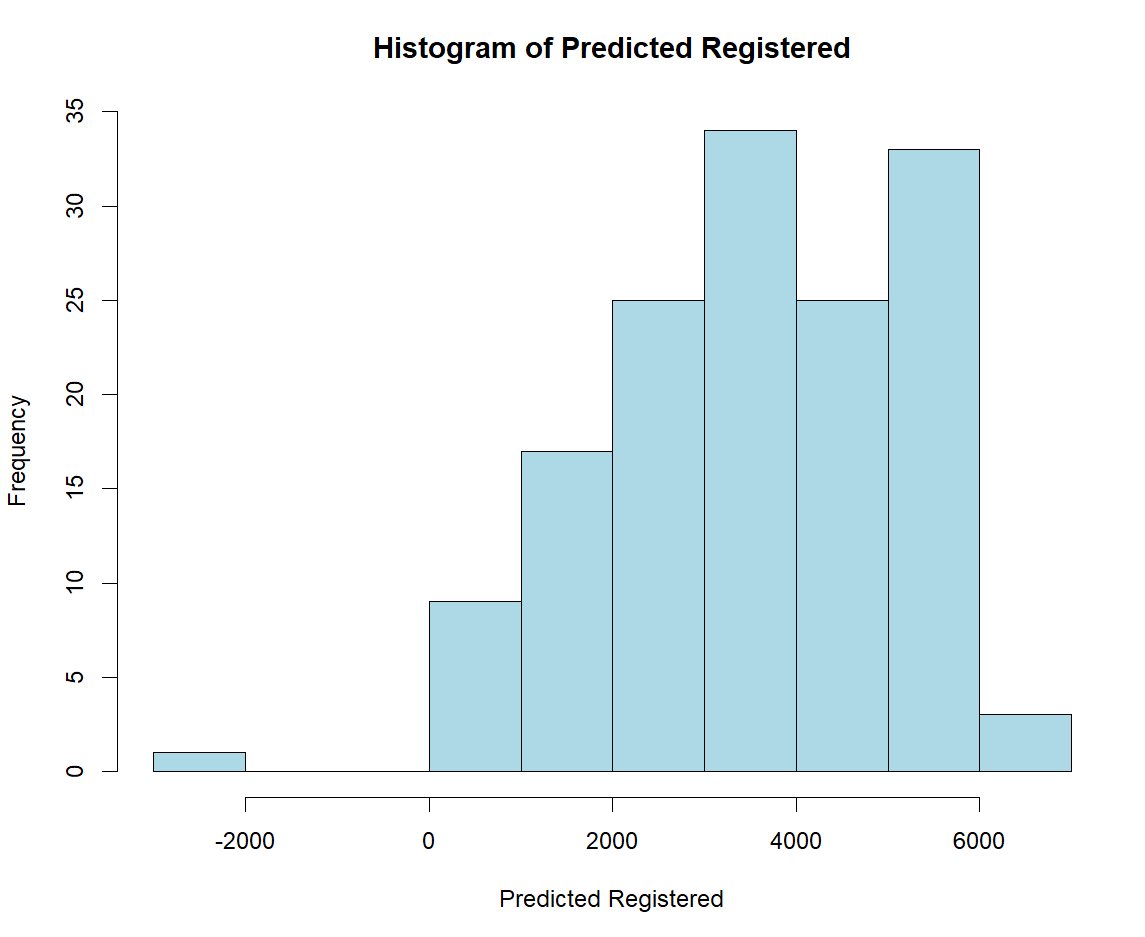
\includegraphics[width=0.7\textwidth]{img/h1b22.png}
\label{fig:scaled_revenue_distribution}
\end{figure}

We compare this to registered, here is the scatter plot of them:

\begin{figure}[H]
\centering
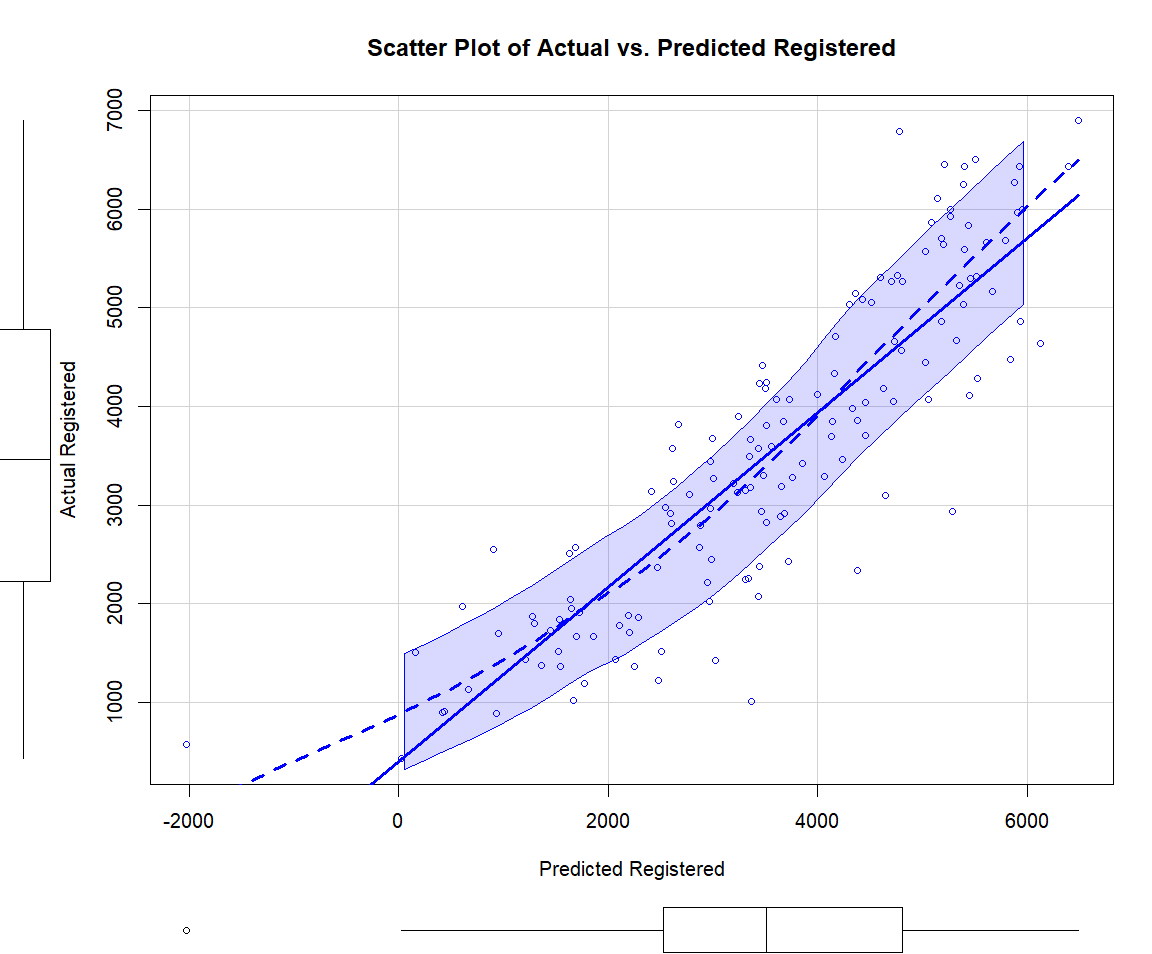
\includegraphics[width=0.7\textwidth]{img/h2b22.png}
\label{fig:scaled_revenue_distribution}
\end{figure}

As they form a almost 45 degree line in the diagonal of the graph, we can say that our model have predict the value of mpg pretty closely.

\subsection{Model Meaning}

Our model is capable of estimating the number of registered bike rentals based on several parameters: holiday, year, weather situation, temperature, humidity, windspeed, and their interactions with month and season. Since the year is used as a continuous variable, this model can also be used for future predictions, though the accuracy may need to be reexamined for future years.

Overall, here is our final model:

\begin{center}
$
M: \ registered \ = \ \beta_1 \ + \ \beta_2 \ holiday \ + \ \beta_3 \ yr \ + \ \beta_{4, j} \ weathersit_j \ + \ \beta_5 \ temp \ + \ \beta_6 \ hum \ + \ \beta_7 \ windspeed \ + \ \beta_{8, k} \ (temp \times season_k) \ + \ \beta_{9, i} \ (temp \times mnth_i) \ + \ \beta_{10, i} \ (hum \times mnth_i) \ + \ \beta_{11, j} \ (hum \times weathersit_j) \ + \ \epsilon
$
\end{center}

With:

\begin{center}
    \begin{align*}
    \beta_1 & = 1727.34 \\
    \beta_2 & = -954.56 \\
    \beta_3 & = 1717.52 \\
    \beta_4 & = 
        \begin{cases} 
          1253.98 & \text{(weathersit2)} \\
          -4887.25 & \text{(weathersit3)} 
        \end{cases} \\
    \beta_5 & = 2806.06 \\
    \beta_6 & = -1103.72 \\
    \beta_7 & = -1923.17 \\
    \beta_8 & = 
        \begin{cases} 
          2377.63 & \text{(temp $\times$ season2)} \\
          2734.72 & \text{(temp $\times$ season3)} \\
          3958.73 & \text{(temp $\times$ season4)} 
        \end{cases} \\
    \beta_9 & = \text{varies by month (temp $\times$ mnth)} \\
    \beta_{10} & = \text{varies by month (hum $\times$ mnth)} \\
    \beta_{11} & = \text{varies by weather situation (hum $\times$ weathersit)} \\
    \end{align*}
\end{center}

Variable meanings:

\begin{itemize}
    \item registered: Number of registered bike rentals.
    \item holiday: 1 if the day is a holiday, 0 otherwise.
    \item yr: Year (0 for 2011, 1 for 2012).
    \item weathersit: Categorical variable representing the weather situation.
    \item temp: Normalized temperature in Celsius.
    \item hum: Normalized humidity.
    \item windspeed: Normalized windspeed.
    \item season: Categorical variable representing the season.
    \item mnth: Categorical variable representing the month.
\end{itemize}

This means that:

\begin{itemize}
    \item The base number of registered bike rentals, when all other variables are at their base levels, is 1727.34.
    \item If the day is a holiday, the number of registered rentals decreases by 954.56.
    \item An increase in the year variable (from 2011 to 2012) increases the number of rentals by 1717.52.
    \item Different weather situations have varying impacts, with `weathersit2` increasing rentals by 1253.98 and `weathersit3` decreasing rentals by 4887.25.
    \item As temperature increases, rentals increase by 2806.06 units.
    \item Higher humidity tends to decrease rentals, but this effect varies by month and weather situation.
    \item Higher windspeed significantly reduces the number of rentals by 1923.17 units.
    \item The interaction effects show that temperature and humidity have different impacts depending on the season, month, and weather situation.
\end{itemize}

In layman's terms, this means:

\begin{itemize}
    \item Registered bike rentals are higher in the year 2012 compared to 2011.
    \item Holidays see fewer bike rentals.
    \item Good weather (as represented by `weathersit2`) increases rentals, while bad weather (`weathersit3`) significantly reduces them.
    \item Warmer days generally lead to more bike rentals.
    \item High humidity and windspeed can decrease the number of rentals.
\end{itemize}

Please note that these conclusions are based on the dataset used and may not fully represent real-world conditions. However, within the scope of our data, the model accurately estimates the number of registered bike rentals.
